\documentclass[letterpaper,11pt,nointlimits,reqno]{amsart}

% Packages
\usepackage{accents}
\usepackage{enumerate}
\usepackage{fancyhdr}
\usepackage[final]{graphicx}
\usepackage{fullpage}
\usepackage{lastpage}
\usepackage{listings}
\usepackage{mathrsfs}
\usepackage{mathtools}
\usepackage[numbers,sort&compress]{natbib}
\usepackage{parskip}
\usepackage{setspace}
\usepackage[usenames,dvipsnames,svgnames,table]{xcolor}

% In conjunction with -shell-escape, automatically convert EPS to PDF
\usepackage{epstopdf}
\epstopdfsetup{outdir=./,suffix=-generated,update,verbose}
\epstopdfDeclareGraphicsRule{.eps}{pdf}{.pdf}{%
    epstopdf --outfile=\OutputFile \space `kpsewhich \space "\SourceFile"`
}

% Hyperref package must be last otherwise the contents are jumbled
% hypertexnames disabled to fix links pointing to incorrect locations
\usepackage[hypertexnames=false,final]{hyperref}

\mathtoolsset{showonlyrefs,showmanualtags}
% \allowdisplaybreaks[1] % Allow grouped equations to be split across pages

% Line Spacing
\singlespacing

% Set appropriate header/footer information on each page
\fancypagestyle{plain}{
    \fancyhf{}
    \renewcommand{\headheight}{2.0em}
    \renewcommand{\headsep}{0.75em}
    \renewcommand{\headrulewidth}{1.0pt}
    \renewcommand{\footrulewidth}{0pt}
    \lhead{
        Favorable pressure gradient base flow computations
    }
    \rhead{
        Page \thepage{} of \pageref{LastPage}
    }
}
\pagestyle{plain}

% Document-specific commands
\newcommand{\Mach}[1][]{\ensuremath{\mbox{Ma}_{#1}}}

\begin{document}

This document discusses how to obtain a favorable pressure gradient base flow
for use within temporally-homogenized boundary layer simulations.  First, a
compressible potential flow problem is formulated for a radially-symmetric
source or sink flow.  This one-dimensional problem is cast into a form
commodity ODE integrators can solve to obtain primitive state as a function of
radius.  The solution is then mapped from $\left(r,\theta\right)$ into
$\left(x,y\right)$ coordinates and a base flow profile taken from some constant
$x$ line segment.  The segment chosen, as well as the radial problem boundary
conditions used, are taken to match some boundary layer edge state of interest.
Curve fits are created from that data and supplied as base flow coefficients
within simulation restart files.

\section{The nondimensional, compressible potential flow equation}

A particularly crisp derivation of the coordinate-independent,
velocity-potential formulation for the compressible potential flow equations
appears in section II.A of \citet{Saad2011Coordinate}.  Decomposing the
dimensional velocity $\vec{u}$ into a scalar and vector potential and assuming
that the flow is irrotational,
\begin{align}
  \vec{u} &= \vec{\nabla}\phi + \vec{\nabla}\times\vec{A} =  \vec{\nabla}\phi
.
\end{align}
Inserting the scalar potential into the continuity equation and assuming
smoothness,
\begin{align}
  0 &= \vec{\nabla}\cdot\rho\vec{u}
     = \vec{\nabla}\cdot\rho\vec{\nabla}\phi
     = \rho\vec{\nabla}^2\phi
     + \vec{\nabla}\rho\cdot\vec{\nabla}\phi
.
\end{align}
From the definition of the speed of sound $a$ notice
\begin{align}
    \frac{\mathrm{d}p}{\mathrm{d}\rho} = a^2
    &\implies
    \vec{\nabla}\rho = \frac{1}{a^2} \vec{\nabla} p
\label{eq:gradrho_gradp_relationship}
.
\end{align}
In a steady, inviscid, irrotational context the momentum equation yields
\begin{align}
    \vec{\nabla}p
    &= -\rho \vec{u}\cdot\vec{\nabla}\vec{u}
     = -\rho \left(   \frac{1}{2}\vec{\nabla}\vec{u}^2
                    - \vec{u}\times\vec{\nabla}\times\vec{u}
        \right)
     = - \frac{1}{2} \rho \vec{\nabla}\vec{u}^2
\label{eq:momentum}
.
\end{align}
Rearranging the continuity result followed by two straightforward substitutions
shows
\begin{align}
    \vec{\nabla}^2\phi
    &= -\vec{\nabla}\phi\cdot\frac{1}{\rho}\vec{\nabla}\rho
     = -\vec{\nabla}\phi\cdot\frac{1}{\rho{}a^2}\vec{\nabla}p
     =  \vec{\nabla}\phi\cdot\frac{1}{2a^2} \vec{\nabla}\vec{u}^2
.
\end{align}
Moving the denominator to the left hand side and inserting the scalar
potential,
\begin{align}
    2 a^2 \vec{\nabla}^2\phi
    &= \vec{\nabla}\phi\cdot \vec{\nabla}\vec{u}^2
     = \vec{\nabla}\phi\cdot \vec{\nabla}\left(\vec{\nabla}\phi\right)^2
\label{eq:cpfgibbs_nothermo_dim}
.
\end{align}

Next, \citeauthor{Saad2011Coordinate} employ that stagnation energy stays
constant throughout such a flow to connect the local speed of sound to
reference parameters and the local velocity.  That is, for flow enthalpy $h =
a^2 / \left(\gamma-1\right)$, reference enthalpy $h_0 = a_0^2 /
\left(\gamma_0-1\right)$, and reference velocity $\vec{u}_0$
\begin{align}
        \frac{a^2  }{\gamma  -1} + \frac{1}{2} \vec{u}^2
     &= \frac{a_0^2}{\gamma_0-1} + \frac{1}{2} \vec{u}_0^2
\end{align}
holds everywhere. From this energy constraint
\begin{align}
        2a^2
     &=   2a_0^2 \frac{\gamma-1}{\gamma_0-1}
        + \left(\gamma-1\right)\vec{u}_0^2
        - \left(\gamma-1\right)\vec{u}^2
\label{eq:stagnation_sound}
\end{align}
may be used within~\eqref{eq:cpfgibbs_nothermo_dim} to produce
\begin{align}
    \left[
          2a_0^2 \frac{\gamma-1}{\gamma_0-1}
        + \left(\gamma-1\right)
          \left(\vec{u}_0^2 - \left(\vec{\nabla}\phi\right)^2\right)
    \right] \vec{\nabla}^2\phi
     = \vec{\nabla}\phi\cdot \vec{\nabla}\left(\vec{\nabla}\phi\right)^2
\label{eq:cpfgibbs_dim}
.
\end{align}
Realizability requires $a^2>0$ causing constraint~\eqref{eq:stagnation_sound}
to imply that globally
\begin{align}
  u^2 &< \frac{2 a_0^2}{\gamma_0 - 1} + u_0^2
\label{eq:stagnation_sound_realizability}
.
\end{align}

To nondimensionalize, chose some reference length $l_0$ and declare
\begin{align}
    x     &= x^\ast l_0
&   u     &= u^\ast u_0
&   a     &= a^\ast a_0
&   \phi  &= \phi^\ast u_0 l_0
&   \rho  &= \rho^\ast \rho_0
&   p     &= p^\ast \rho_0 a_0^2
\label{eq:nondimensionalization}
\end{align}
where starred quantities are dimensionless.  Inserting the definitions
into~\eqref{eq:cpfgibbs_dim},
\begin{align}
    \left[
          2a_0^2 \frac{\gamma-1}{\gamma_0-1}
        + u_0^2 \left(\gamma-1\right)
          \left(1 - \left(\vec{\nabla}^\ast\phi^\ast\right)^2\right)
    \right] \frac{u_0}{l_0} {\vec{\nabla}^\ast}^2\phi^\ast
     =       \frac{u_0^3}{l_0} \vec{\nabla}^\ast\phi^\ast
       \cdot \vec{\nabla}^\ast\left(\vec{\nabla}^\ast\phi^\ast\right)^2
.
\end{align}
Multiplying by $\frac{l_0}{a_0^2 u_0}$, identifying $\Mach =
\frac{u_0}{a_0}$, and dropping the star notation,
\begin{align}
    \left[
          2 \frac{\gamma-1}{\gamma_0-1}
        + \Mach^2 \left(\gamma-1\right)
          \left(1 - \left(\vec{\nabla}\phi\right)^2\right)
    \right] {\vec{\nabla}}^2\phi
     =       \Mach^2 \vec{\nabla}\phi
       \cdot \vec{\nabla}\left(\vec{\nabla}\phi\right)^2
.
\end{align}
Moving the $\Mach^2$ term to the right hand side, rescaling, and distributing,
\begin{align}
       {\vec{\nabla}}^2\phi
    &= \frac{\Mach^2}{2}\frac{\gamma_0-1}{\gamma-1} \left(
         \vec{\nabla}\phi \cdot \vec{\nabla}\left(\vec{\nabla}\phi\right)^2
       +
       \left[
             \left(\gamma-1\right)
             \left(\left(\vec{\nabla}\phi\right)^2 - 1\right)
       \right] {\vec{\nabla}}^2\phi
       \right)
\\  &= \frac{\Mach^2}{2} \left(
         \frac{\gamma_0-1}{\gamma-1}
         \vec{\nabla}\phi \cdot \vec{\nabla}\left(\vec{\nabla}\phi\right)^2
       +
       \left[
             \left(\gamma_0-1\right)
             \left(\left(\vec{\nabla}\phi\right)^2 - 1\right)
       \right] {\vec{\nabla}}^2\phi
       \right)
.
\end{align}
This formulation is most useful when $\gamma$ is known or when it can be
connected to $\phi$ in some manner.  Adding a constant $\gamma=\gamma_0$
assumption, one arrives at
\begin{align}
       {\vec{\nabla}}^2\phi
    &=   \frac{1}{2}\Mach^2
         \vec{\nabla}\phi \cdot \vec{\nabla}\left(\vec{\nabla}\phi\right)^2
       +
         \frac{\gamma_0-1}{2}\Mach^2
         \left(\left(\vec{\nabla}\phi\right)^2 - 1\right)
         {\vec{\nabla}}^2\phi
\label{eq:cpfgibbs_nondim}
\end{align}
which is an awfully nonlinear but pleasantly univariate result.

With some $\vec{u}=\vec{\nabla}\phi$ satisfying~\eqref{eq:cpfgibbs_nondim} in
hand, computing local $\rho$ and $p$ is often of interest.
Nondimensionalizing~\eqref{eq:stagnation_sound} permits direct computation of
$a$ from
\begin{align}
  a^2 &= \frac{\gamma-1}{\gamma_0-1}
       + \Mach^2\frac{\gamma-1}{2}\left(1-\vec{u}^2\right)
\label{eq:stagnation_sound_nondim}
.
\end{align}
The nondimensional analogue of
inequality~\eqref{eq:stagnation_sound_realizability} becomes
\begin{align}
  u^2 &< \frac{2}{\Mach^2\left(\gamma_0-1\right)} + 1
.
\label{eq:stagnation_sound_realizability_nondim}
\end{align}
Combining~\eqref{eq:gradrho_gradp_relationship} and~\eqref{eq:momentum} to form
$\vec{\nabla}\rho / \rho$, nondimensionalizing, multiplying by $l_0$, and
simplifying,
\begin{align}
  \vec{\nabla}\log\rho
  &=
  -\frac{\Mach^2}{2}\frac{\vec{\nabla}\vec{u}^2}{a^2}
.
\end{align}
Nondimensionalizing the momentum result~\eqref{eq:momentum} and then scaling by
$\frac{l_0}{\rho_0 a_0^2}$,
\begin{align}
  \vec{\nabla} p &= - \frac{1}{2}\Mach^2 \rho \vec{\nabla}\vec{u}^2
.
\end{align}
Both of the previous two local statements can be made global by integrating
over some domain $\Omega$ and applying a corollary of Gauss' theorem:
\begin{align}
  \int_{\partial\Omega} \log\rho \, \mathrm{d}S
  &=
  - \frac{\Mach^2}{2}\int_{\Omega}
    \frac{\vec{\nabla}\vec{u}^2}{a^2} \, \mathrm{d}x
\label{eq:logrho_nondim}
\\
  \int_{\partial\Omega} p \, \mathrm{d}S
  &=
  - \frac{\Mach^2}{2}\int_{\Omega} \rho \vec{\nabla}\vec{u}^2 \, \mathrm{d}x
\label{eq:p_nondim}
\end{align}


\section{Reduction to the radially-symmetric, two-dimensional case}

Suppose radial symmetry in which $\phi=\phi\left(r\right)$.  \emph{Mathematica}
eases translating~\eqref{eq:cpfgibbs_nondim} into this setting
\\\begin{minipage}{\textwidth} % BEGIN Avoids page break
\begin{lstlisting}[language=Mathematica,columns=flexible,
                   basicstyle={\footnotesize\sffamily},frame=single]
    Needs["VectorAnalysis`"];
    SetCoordinates[Cylindrical];
    With[{f=phi[Rr]},
        With[{gf=Simplify[Grad[f]],lf=Simplify[Laplacian[f]]},
            With[{gf2 = Simplify[DotProduct[gf,gf]]},
                lf-(Ma^2/2) DotProduct[gf,Grad[gf2]]-(gamma0-1)(Ma^2/2)(gf2-1)lf
            ]
        ]
    ];
    Collect[%,{phi''[Rr],phi'[Rr],phi[Rr]}];
    Map[Simplify,%]
\end{lstlisting}
\end{minipage}                 % END   Avoids page break
producing output equivalent to
\begin{align}
    \frac{2+\Mach^2\left(\gamma_0-1\right)}{2 r}\phi^\prime
   -\frac{  \Mach^2\left(\gamma_0-1\right)}{2 r}{\phi^\prime}^3
   +\frac{1}{2}\left(2+\Mach^2\left(\gamma_0-1\right)
                      -\Mach^2\left(\gamma_0+1\right){\phi^\prime}^2\right)
               \phi^{\prime\prime}
   &= 0
.
\end{align}
Rewriting using $u = \phi^\prime(r)$ followed by solving for $u'$,
\begin{align}
   u^\prime
   &=
   -\frac{u}{r}
   \cdot
   \frac{
      2
    + \Mach^2\left(\gamma_0-1\right)
    - \Mach^2\left(\gamma_0-1\right) u^2
   }{
      2
    + \Mach^2\left(\gamma_0-1\right)
    - \Mach^2\left(\gamma_0+1\right) u^2
   }
\label{eq:cpfradial_nondim_ode}
.
\end{align}
With appropriate boundary conditions on some $\left[R_1, R_2\right]$,
equation~\eqref{eq:cpfradial_nondim_ode} allows integrating for $u$.

Given some $u$ one also wants to be able to compute local thermodynamic state.
Equation~\eqref{eq:stagnation_sound_nondim} fixes $a$.  The $\phi=\phi(r)$
assumption causes~\eqref{eq:logrho_nondim} to become
\begin{align}
  \rho\!\left(R_2\right)
  &=
  \exp\left[
    - \frac{\Mach^2}{2} \int_{R_1}^{R_2}
        \frac{\left(u^2\right)'}{a^2}
      \, r \, \mathrm{d}r
    + \log\rho\!\left(R_1\right)
  \right]
\\
  &=
  \rho\!\left(R_1\right) \exp\left[
    - \Mach^2 \int_{R_1}^{R_2}
        \frac{u u'}{a^2}
      \, r \, \mathrm{d}r
  \right]
\label{eq:cpfradial_nondim_rho}
.
\end{align}
Likewise~\eqref{eq:p_nondim} simplifies to
\begin{align}
  p\!\left(R_2\right)
  &=
    - \frac{\Mach^2}{2} \int_{R_1}^{R_2}
        \rho \left(u'\right)^2
      \, r \, \mathrm{d}r
    + p\!\left(R_1\right)
\\
  &=
    -\Mach^2 \int_{R_1}^{R_2} \rho u u' \, r \, \mathrm{d}r
      + p\!\left(R_1\right)
\label{eq:cpfradial_nondim_p}
.
\end{align}
Notice~\eqref{eq:cpfradial_nondim_ode} easily supplies $u'$ for the computation
of both $\rho$ and $p'$.

\section{The radially-symmetric sub- and supersonic nozzle problems}

Equations~\eqref{eq:cpfradial_nondim_ode}, \eqref{eq:cpfradial_nondim_rho}
and~\eqref{eq:cpfradial_nondim_p} may be used to find solutions to idealized
sub- and supersonic radial nozzle and diffuser problems.  In particular,
obtaining a favorable pressure gradient, i.e. one where
$\frac{\mathrm{d}p}{\mathrm{d}r} < 0$, requires imposing boundary conditions
for sub- and supersonic nozzles.  Many texts, e.g.
\citet[\textsection{}9.4]{White1999Fluid} and
\citet[\textsection{}97]{Landau2004Fluid}, cover the simpler case when the area
changes slowly as one progresses downstream in the device.  In contrast, this
treatment produces geometries violating that requirement.

A subsonic nozzle may be posed on nondimensional~$\left[R_{1}, R_{2}\right]$ by
setting inflow per
\begin{align}
    -a_0 < u\!\left(l_0 R_{2}\right) u_0 < 0
    &\implies
    u\!\left(R_{2}\right) \in \left(-\Mach^{-1}, 0\right)
.
\end{align}
With this condition, $-u$ increases and $p$ decreases when traversing the
domain from~$R_{2}$ to~$R_{1}$.  However, the problem becomes stiff as the flow
approaches sonic conditions.  A workaround is specifying at most a sonic
outflow via
\begin{align}
    -a_0 < u_0 u\!\left(l_0 R_1\right) < 0
    &\implies
    u\!\left(R_1\right) \in \left(-\Mach^{-1}, 0\right)
\label{eq:cpfradial_nozzle_subsonic_bc}
\end{align}
in conjunction with taking $R_{2}$ large enough to obtain the desired upstream
$u\!\left(R_{2}\right)$ condition.  Caveat numerical errors, specifying either
the inflow or outflow condition is equivalent as the physics are frictionless.

A supersonic nozzle may be posed on nondimensional~$\left[R_{1}, R_{2}\right]$
by setting inflow
\begin{align}
    u_0 u\!\left(l_0 R_{1}\right) > a_0 > 0
    &\implies
    u\!\left(R_{1}\right) \in \left(\Mach^{-1}, \infty\right)
\label{eq:cpfradial_nozzle_supersonic_bc}
.
\end{align}
In this situation, $u$ increases and $p$ decreases when traversing the domain
from~$R_{1}$ to~$R_{2}$.  As above, a supersonic outflow could instead be
specified at $R_{2}$.

Working with boundary conditions~\eqref{eq:cpfradial_nozzle_subsonic_bc}
and~\eqref{eq:cpfradial_nozzle_supersonic_bc} on $\left[R_1, R_2\right]$ in
conjunction with~\eqref{eq:cpfradial_nondim_ode} presents initial value
problems amenable to solution by numerical ODE integrators.  For example,
\texttt{Octave}\citep{Eaton2008GNU} armed with the \texttt{odepkg} package can
solve such problems.  A straightforward implementation appears in
Listing~\ref{lst:octave_nozzle1} with demo logic producing the solutions
depicted in Figure~\ref{fig:sample_solns}.  While
Listing~\ref{lst:octave_nozzle1} is succinct, its $\rho$ and $p$ solution
accuracies are not controlled in the same manner its $u$ accuracy.  By coupling
the integration of $u'$, $\left(\log\rho\right)'$, and $p'$ one may achieve
higher order behavior with an implementation like
Listing~\ref{lst:octave_nozzle}.

\lstinputlisting[language=Octave,columns=fixed,float=p,
                 caption={\texttt{nozzle1.m}: A scalar-by-scalar radial
                 nozzle solver implementation\label{lst:octave_nozzle1}},
                 basicstyle={\footnotesize\sffamily},frame=single]
                {notebooks/nozzle1.m}

\begin{figure}[p]
  \centering
  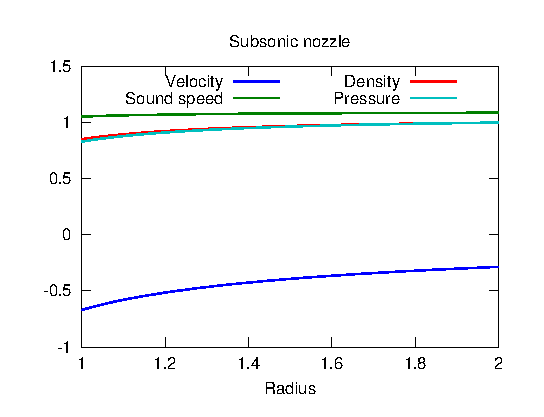
\includegraphics[width=0.80\textwidth]{nozzle_subsonic}
  \vfill
  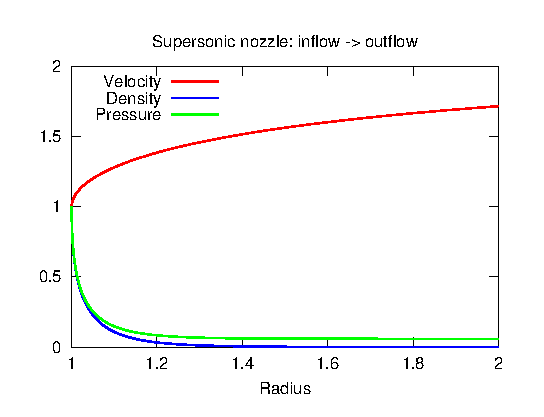
\includegraphics[width=0.80\textwidth]{nozzle_supersonic}
  \caption{
      \label{fig:sample_solns}
      Sample solutions saved by the demo logic in \texttt{nozzle1.m}.  The
      subsonic case flows from right-to-left while the supersonic one flows
      from left-to-right.
  }
\end{figure}

\lstinputlisting[language=Octave,columns=fixed,float=p,
                 caption={\texttt{nozzle.m}: A higher-order, ``coupled''
                 radial nozzle solver
                 implementation\label{lst:octave_nozzle}},
                 basicstyle={\footnotesize\sffamily},frame=single]
                {notebooks/nozzle.m}

\clearpage

\section{Mapping solution to Cartesian domain and matching conditions of interest}

\begin{figure}[h]
  \centering
  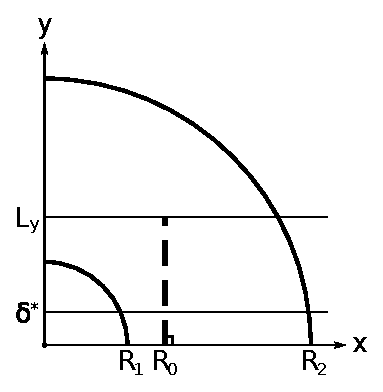
\includegraphics[width=0.30\textwidth]{nozzle_schematic}
  \caption{
      \label{fig:mapping_geometry}
      The geometry used when extracting base flow profiles
  }
\end{figure}

The favorable pressure gradient base flow profile of height $L_y$ is taken from
a constant $x$ line segment obtained from a radially-varying solution.
Referring to Figure~\eqref{fig:mapping_geometry}, the solution comprised of
$u\!\left(R\right)$, $p'\!\left(R\right)$, and $a\!\left(R\right)$ is valid for
$R\in\left[R_1,R_2\right]$.  For some $R_0$, a profile is gathered from the
line segment between Cartesian points $\left(R_0,0\right)$ and
$\left(R_0,L_y\right)$.  Clearly, selecting
\begin{align}
  R_1 &= R_0
&
  R_2 &= \sqrt{R_0^2 + L_y^2}
\end{align}
produces the smallest domain possessing a solution along this entire segment.

At some height of interest, say an edge distance $\delta$ from the $x$-axis,
one can evaluate
\begin{align}
  \Mach[e]{}
  &\equiv
  \left. \frac{u_0 u\cdot\hat{\xi}}{a_0 a} \right|_{\left(R_0,\delta\right)}
  =
  \left.
    \frac{\Mach R_0}{R}
    \frac{\left|u\!\left(R\right)\right|}
         {      a\!\left(R\right)       }
  \right|_{R = \sqrt{R_0^2 + \delta^2}}
\end{align}
\begin{align}
  p_{e,\xi}
  &\equiv
  \left.
  \frac{l_0 \delta}{\rho_0 \rho \, u_0^2 u^2}
    \frac{\mathrm{d}\left(p_0 p\right)}{\mathrm{d}\left(l_0 \xi\right)}
  \right|_{\left(R_0,\delta\right)}
  =
  \left.
    \frac{\operatorname{sgn}(u) \, \delta}{\Mach^2 \rho u^2}
      \frac{\mathrm{d}p}{\mathrm{d}x}
  \right|_{\left(R_0,\delta\right)}
  =
  \left.
    \frac{\operatorname{sgn}(u) R \, \delta \, p'\!\left(R\right)}
         {\Mach^2 R_0 \, \rho\!\left(R\right) u^2\!\left(R\right)}
  \right|_{R=\sqrt{R_0^2 + \delta^2}}
\end{align}
to interrogate the local solution nature at $\left(R_0, \delta\right)$.  Here,
$\hat{\xi}$ denotes $\hat{x}$ with the streamwise direction defined to be
positive.  The squared sound speed at $y=\delta$ and $y=0$ is
\begin{align}
  a^2_e
  &\equiv
  a^2\!\left(\sqrt{R_0^2 + \delta^2}\right)
,
&
  a^2_w
  &\equiv
  a^2\!\left(R_0\right)
.
\end{align}
In the special case of a thermally and calorically perfect gas, these are
nothing but temperatures $T_e$ and $T_w$ because
choices~\eqref{eq:nondimensionalization} imply $a^2 = T$ holds in that
particular context.  A kernel building atop Listing~\ref{lst:octave_nozzle}.
to compute these quantities of interest appears in
Listing~\ref{lst:octave_nozzle_qoi}.  The kernel takes $R_2 = \sqrt{R_0^2 +
\delta^2}$ to speed the computation and to causes the ODE integrator to
automatically produce full-order results at $\left(R_0,\delta\right)$ without
requiring dense output capabilities.

\lstinputlisting[language=Octave,columns=fixed,float,
                 caption={\texttt{nozzle\_qoi.m}: A kernel computing several
                 nozzle quantities of interest\label{lst:octave_nozzle_qoi}},
                 basicstyle={\footnotesize\sffamily},frame=single]
                {notebooks/nozzle_qoi.m}

A nonlinear optimization problem may be formulated over $\Mach$, $R_0$,
$\rho\!\left(R_1\right)$, and $u\!\left(R_1\right)$ to match some target
$\Mach[e]{}$, $p_{e,\xi}$, and $T_e$ given fixed $\delta$ and $\gamma_0$.
Parameter $p\!\left(R_1\right)$ may be arbitrarily fixed as it does not impact
these particular target quantities.  One possible implementation, written using
the \texttt{nonlim\_resid} method from \texttt{Octave}'s \texttt{optim}
package, is given in Listing~\ref{lst:octave_nozzle_baseflow}.  Several choices
are worth noting:
\begin{enumerate}
  \item The relative residuals are minimized rather than the absolute residuals
    as otherwise the larger magnitudes of $\Mach[e]{}$ swamp $p_{e,\xi}$
    producing undesirable results.
  \item To combat the impact of a poor initial guess, optimization proceeds in
    two phases with the first phase treating only $R_0$ and
    $u\!\left(R_1\right)$ as free parameters.
  \item As shown, $\rho\!\left(R_1\right)$ is taken fixed because because, for
    it to have appreciable impact on the optimization results, the parameter
    often take physically unsatisfying values for an order-one nondimensional
    quantity.
\end{enumerate}
After optimization completes, the full base flow profile may be computed by
supplying $R_2 = \sqrt{R_0^2 + L_y^2}$ to the routine in
Listing~\ref{lst:octave_nozzle}.

\lstinputlisting[language=Octave,columns=fixed,%NO float,
                 caption={\texttt{nozzle\_baseflow.m}: A driver for targeting
                 quantities of interest\label{lst:octave_nozzle_baseflow}},
                 basicstyle={\footnotesize\sffamily},frame=single]
                {notebooks/nozzle_baseflow.m}

\newcommand*{\doi}[1]{\href{http://dx.doi.org/\detokenize{#1}}{doi: #1}}
\bibliographystyle{plainnat}
\bibliography{references}

\end{document}
